% VUT FIT MITAI
% MSZ 2021/2022
% Author: Vladimir Dusek
% Login: xdusek27

%%%%%%%%%%%%%%%%%%%%%%%%%%%%%%%%%%%%%%%%%%%%%%%%%%%%%%%%%%%%%%%%%%%%%%%%%%%%%%%%

% Path to figures
\graphicspath{{upa/prostorove_db_indexace/figures}}

%%%%%%%%%%%%%%%%%%%%%%%%%%%%%%%%%%%%%%%%%%%%%%%%%%%%%%%%%%%%%%%%%%%%%%%%%%%%%%%%

\chapter{UPA~--~Indexace (nejen) v prostorových DB (kD-Tree a Grid File (a jejich varianty), R-Tree).}

%%%%%%%%%%%%%%%%%%%%%%%%%%%%%%%%%%%%%%%%%%%%%%%%%%%%%%%%%%%%%%%%%%%%%%%%%%%%%%%%

\section{Zdroje}

\begin{compactitem}
    \item \path{PDB-Spatial-CZ.pdf}
    \item \path{03-spatial_databases.pdf}
    \item \path{szz-kastak.pdf}
    \item \path{szz-discord-bazi.pdf}
\end{compactitem}

%%%%%%%%%%%%%%%%%%%%%%%%%%%%%%%%%%%%%%%%%%%%%%%%%%%%%%%%%%%%%%%%%%%%%%%%%%%%%%%%

\section{Úvod a kontext}

\begin{compactitem}
    \item Ve vícedimenzionálním prostoru nelze z reprezentace hodnot jednoznačně určit uspořádání -- předchůdce a následníka. Nelze tedy použít obecně užívané indexační algoritmy pro 1D.

    \item Řešením by mohlo být mapování bodů do jediné dimenze, nicméně zde dochází ke ztrátě sousednosti, transformace by nemusela být realizovatelná a výsledek dotazů by nemusel být transformovatelný zpět.

    \item Z tohoto důvodu se v prostorových databázích využívají specializované indexační algoritmy.
\end{compactitem}

%%%%%%%%%%%%%%%%%%%%%%%%%%%%%%%%%%%%%%%%%%%%%%%%%%%%%%%%%%%%%%%%%%%%%%%%%%%%%%%%

\section{Indexace bodů}

\subsection{Stromy dělící prostor}

\subsubsection{k-D Tree}

\begin{compactitem}
    \item k-D Tree je datová struktura (binární strom) dělící prostor hyperplochami na nejvyšší možné úrovni, a to vždy na dvě části. \begin{compactitem}
        \item Hyperplocha v rovině to je přímka.
        \item Dělící hyperplocha musí být rovnoběžná s osovým (souřadným) systémem.
    \end{compactitem}

    \item Myšlenka: vytvoříme uspořádání na množině bodů v prostoru (podobně jako ho máme přirozeně na množině čísel) a díky tomu, budeme moct uspořádat body do stromu.

    \item Při dělení, musí ve výsledných plochách být obsažen vždy aspoň jeden bod, který pak už není součástí jakékoli jiné hyperplochy.

    \item Vkládání a vyhledávání je bez problému, avšak při mazání je potřeba znovuustavit celý strom, algoritmus je tak vhodný pro statická data.
\end{compactitem}

\begin{figure}[H]
    \centering
    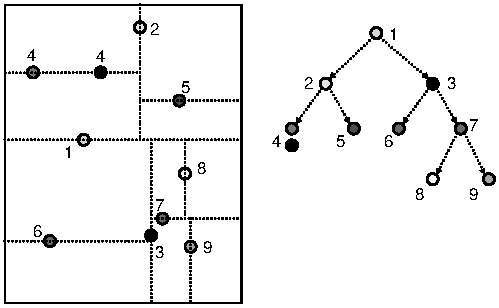
\includegraphics[width=0.75\linewidth]{kd_tree.pdf}
    \caption{k-D tree.}
\end{figure}

\subsubsection{Adaptivní k-D Tree}

\todo{todo}

\begin{figure}[H]
    \centering
    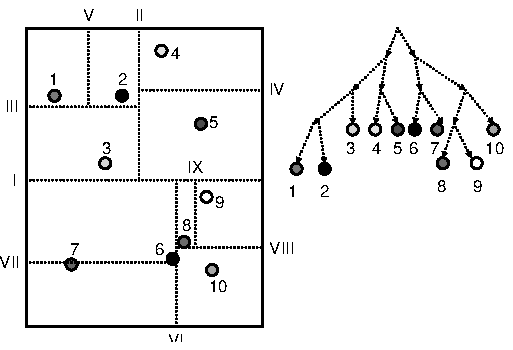
\includegraphics[width=0.75\linewidth]{adaptivni_kd_tree.pdf}
    \caption{Adaptivní k-D Tree.}
\end{figure}

\subsubsection{BSP Tree}

\todo{todo}

\begin{figure}[H]
    \centering
    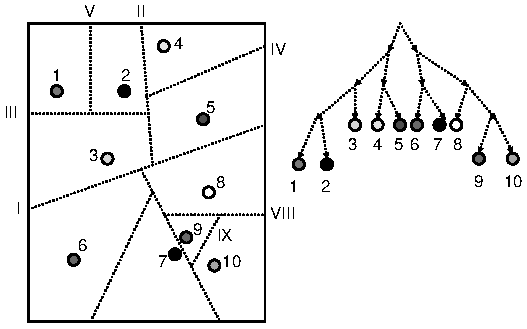
\includegraphics[width=0.75\linewidth]{bsp_tree.pdf}
    \caption{BSP Tree.}
\end{figure}

\subsubsection{Quad Tree}

\todo{todo}

\begin{figure}[H]
    \centering
    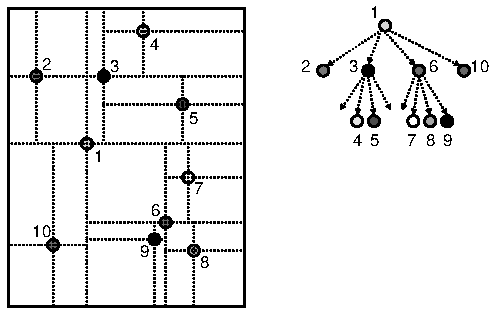
\includegraphics[width=0.75\linewidth]{quad_tree.pdf}
    \caption{Quad Tree.}
\end{figure}

\subsection{Hashování}

Grid File

Two-level Grid File

\todo{todo}

%%%%%%%%%%%%%%%%%%%%%%%%%%%%%%%%%%%%%%%%%%%%%%%%%%%%%%%%%%%%%%%%%%%%%%%%%%%%%%%%

\section{Indexace objektů}

\todo{todo}

\subsection{Překrývání (overlapping)}

R-Trees

$\text{R}^*$-Trees

\subsection{Ořezávání (clipping)}

$\text{R}^+$-Trees
